\documentclass{article}
\usepackage[]{algorithm2e}
\SetKw{Assert}{assert}
\usepackage{drawstack}

\usepackage[framemethod=tikz]{mdframed}
\mdtheorem[linecolor=blue,frametitlerule=true]{definition}{Definition}
\mdtheorem[linecolor=red,frametitlerule=true]{example}{Exampl}

\usepackage{marginnote}
\usepackage[outer=4.5cm, marginparwidth=3cm, marginparsep=0.5cm]{geometry}
\usepackage{tikz}
\usepackage[utf8]{inputenc}
\usepackage{listings}
\lstset{tabsize=2}
\definecolor{lightred}{rgb}{1,0.9,0.9}
\lstset{backgroundcolor=\color{lightred}}
%\lstset{numbers=left}


\usepackage{VassorTitle}

\institution{École polytechnique fédérale de Lausanne}
\title{Verified double-hashing hash map}
\supervisor{G. \textsc{Candea}, Pr.\\
K. \textsc{Argyraki}, Pr.\\
A. \textsc{Zaostrovnykh}, Ph. D. Student}
\project{Optionnal Semester Project}
\author{Martin \textsc{Vassor}}
\date{\today}

\newcommand{\keyvalue}[2] {
	\begin{tabular}{| p{0.8cm} | p{1.3cm} |}
			\hline
			\texttt{#1} & \texttt{#2} \\
			\hline
		\end{tabular}
}

\begin{document}
\maketitle
\section{Introduction}
\section{Implementation}


\section{Verification}

\subsection{Provided proof}
\subsubsection{Requirement (\texttt{R})}
\marginnote{\texttt{up\_to(nat, prop)} verifies that \texttt{prop} is ensured for all \texttt{i} below \texttt{nat}: \\
\texttt{up\_to(0, prop) = true}\\
\texttt{up\_to(n, prop) = prop(n-1) \&\& up\_to(n-1, prop)}}
Figure~\ref{fig:for_loop_orig_pruned} present the relevant part of the proof of the original loop in \texttt{find\_key}. The last statement (\texttt{no\_key\_found(ks, k)}) requires the property \texttt{not\_my\_key(k)} to be verified for all current keys in the mapping, ensured by the \texttt{up\_to(nat\_of\_int(length(ks)), \ldots(not\_my\_key)(k)\ldots)} statement.

This \texttt{up\_to} statement is proved by the \emph{for}-loop invariant: at each round, \texttt{not\_my\_key(k, nth(index, ks))} is ensured, either because the cell is empty (\texttt{no\_busy\_no\_key} lemma), either because the hash does not match (\texttt{no\_hash\_no\_key} lemma), either because the key does not match (hence inferred by Verifast). 

Finally, the \emph{for}-loop only proves that the \texttt{up\_to} statement holds when starting from \texttt{index = start} and looping. The lemma \texttt{by\_loop\_for\_all} prove that this loop access is equivalent to a continuous access from \texttt{0} to \texttt{length}.

\begin{figure}[b]
	\lstinputlisting[language=C]{for_loop_orig_pruned.c}
	\caption{Original \emph{for}-loop for searching a key}
	\label{fig:for_loop_orig_pruned}
\end{figure}

\subsubsection{Impact of the modifications}
TODO


\subsection{The \texttt{stripe\_l\_fp} fixpoint}
\subsubsection{Definition}

First, a fixpoint is defined, which returns the index to be updated after $n$ iterations with an offset of $step$, starting from $start$ with capacity $capa$. 
\marginnote{A lemma ensuring that $\mathtt{stripe} = start + n*step \% capa$ is proved.}
\begin{definition}[stripe(int start, int step, nat n, int capa)]
	\begin{lstlisting}
fixpoint int stripe(int start, int step, nat n, int capa) {
	switch(n) {
		case zero: return start;
		case succ(m): return 
			(stripe(start, step, m, capa) + step) % capa;
	}
}
	\end{lstlisting}
	
\end{definition}

The \texttt{stripe\_l\_fp} fixpoint builds a \texttt{list<option<nat>>} given a starting point, an offset, a number of accesses and a capacity. The base case of this fixpoint is to generate a \texttt{list} containing only \texttt{none}s (fixpoint \texttt{gen\_none}), if \texttt{zero} accesses are performed. The recursive case is to update the $start + n*offset \%capa$ cell, using the above \texttt{stripe} fixpoint.

\begin{definition}[stripe\_l\_fp(int start, int step, nat bound, int capa)]
	\begin{lstlisting}
fixpoint list<option<nat> > stripe_l_fp(int start,
	int step, nat n, int capa)
{
	switch(n) {
		case zero: return gen_none(nat_of_int(capa));
		case succ(m): return update(stripe(start, step, n, capa),
			some(n), stripe_l_fp(start, step, m, capa));
	}
}
 	\end{lstlisting}
\end{definition}

\begin{example}[\texttt{stripe\_l\_fp(0, 2, 5, 7)}]
	Calling \texttt{stripe\_l\_fp(0, 2, 5, 7)} produces the following list. Notice that the base case returns a list containing only \texttt{none}s, not a list containing a \texttt{some(0)}. 
	\begin{center}
		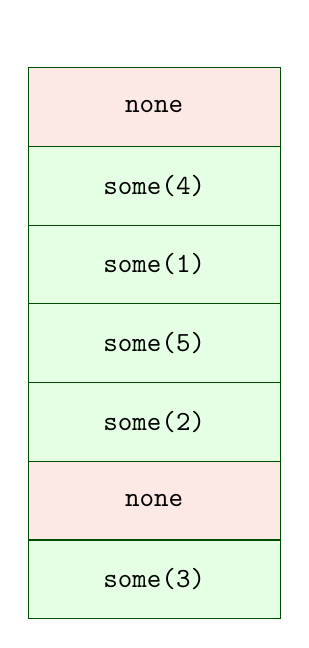
\begin{tikzpicture}
			\drawstruct{(0,0)}
			\structcell[occupiedcell]{\texttt{none}} ;
			\structcell[freecell]{\texttt{some(4)}} ;
			\structcell[freecell]{\texttt{some(1)}} ;
			\structcell[freecell]{\texttt{some(5)}} ;
			\structcell[freecell]{\texttt{some(2)}} ;
			\structcell[occupiedcell]{\texttt{none}} ;
			\structcell[freecell]{\texttt{some(3)}} ;
		\end{tikzpicture}
	\end{center}
\end{example}


\subsubsection{Properties}
The main property required is that the number of cell containing \texttt{some(i)} (for any \texttt{i}) is equal to the number of steps done. This property will later be used to ensures that all cells are eventually reached (see Subsection~\ref{seq:stripe_to_stride}). The function that count the number of such cells is named \texttt{count\_some(list<option<nat>> list)}.

There are also other properties which are used internally to prove the \texttt{count\_some} property. The main lemma is named \texttt{stripe\_l}.

\begin{definition}[Prototype of \texttt{stripe\_l}]
	\begin{lstlisting}
lemma list<option<nat> > stripe_l(int start, int step, nat n, int capa)
requires 0 <= start &*& start < capa &*& step > 0 &*& int_of_nat(n) <= capa &*& coprime(step, capa) &*& step < capa;
ensures count_some(result) == n
&*& length(result) == capa
&*& true == up_to(nat_of_int(capa), (list_contains_stripes)(result, start, step))
&*& true == up_to(nat_of_int(capa), (lst_opt_less_than_n)(result, n))
&*& true == forall(result, opt_not_zero)
&*& result == stripe_l_fp(start, step, n, capa)
&*& coprime(step, capa);
	\end{lstlisting}
\end{definition}

\subsubsection{Proof of \texttt{stripe\_l}}
The proof of these properies relies on the fact that the same cell is not updated twice. Once this is ensured, the construction of the fixpoint ensures the validity of the properties. 

Algorithm~\ref{alg:proof_stripe_l} shows the main steps of the proof. In the base case, all trivially holds. In the inductive case, if the \texttt{stripe(start, step, n, capa)}-th cell (i.e. the one hit at $n$-th iteration) already contains \texttt{some(i)}, the \texttt{list\_contains\_stripes} property ensures that \texttt{stripe(start, step, i, capa)}-th cell is the one we are hitting. Hence, $start + step\times i \%capa = start + step\times n \%capa$, with $n-i < capa$. Then the Chinese remainder theorem leads to a contradiction.

\begin{algorithm}
	\caption{Proof of stripe\_l\label{alg:proof_stripe_l}}

	\KwIn{int start, int step, nat n, int capa}	

	\Switch{n}{
		\Case{zero}{
			\tcp{All hold by construction}
		}
		\Case{succ(m)}{
			\tcp{Recursive call}
			list $lst \longleftarrow \mathtt{stripe\_l(start, step, m, capa)}$
			
			\tcp{Now, we want to update the stripe(start, step, n, capa)-th to some(n)}
			\tcp{Proof by contradiction that the cell contains none}
			\Switch{nth(stripe(start, step, n, capa), lst}{
				\Case{some(i)}{
					\Assert{$start + i\times step \%capa = start + n\times step \%capa$}\;
					\Assert{$(n-i)\times step\%capa = 0$}\;
					\Assert{$n-i < capa$}\;
					\tcp{The chinese remainder theorem applies and shows a contradiction}
					chinese\_remainder\_theorem(step, capa, $(n-i)\times step$)\;
				}
				\Case{none}{
				}
			}
			\tcp{We now that the stripe(start, step, n, capa)-th cell contains a \texttt{none}, which we update to \texttt{some(n)}, so the properties hold for the updated list.}
			\marginnote{The \texttt{update(index, elem, list)} fixpoint returns \texttt{list} with the \texttt{index}-th element updated to \texttt{elem}.}
			\Return{update(stripe(start, step, n, capa), some(n), lst)}
			
		}
	}
\end{algorithm}

\subsubsection{From \texttt{stripe} fixpoint to \texttt{R}}
\label{seq:stripe_to_stride}

\subsection{Proof of the \emph{Chinese remainder theorem}}
\subsubsection{Properties}
\subsubsection{Computation of \emph{gcd}}
\subsubsection{\emph{gcd} properties}
\subsubsection{Proof by contradiction}

\section{Conclusion}
\subsection{Validity of benchmark}
\subsection{Forthcoming work}


\end{document}
